\documentclass[12pt, a4paper]{article}
\usepackage[utf8]{inputenc}
\usepackage{amsmath}
\usepackage{relsize}
\usepackage{array}
\usepackage{xcolor}
\usepackage{courier}
\usepackage{listings}
\lstset{basicstyle=\footnotesize\ttfamily,breaklines=true}
\lstset{framextopmargin=50pt,frame=bottomline}
\usepackage{tikz}
\usetikzlibrary{calc}
\usepackage{graphicx}
\graphicspath{ {./images/} }
\usepackage{multirow}
\usepackage{adjustbox}
\usepackage{amssymb}

\title{CEG3155A Assignment 5}
\author{Jake Wang/*}
\date{\today}

\begin{document}
	\maketitle
	
	\section*{Question I}
	\subsection*{Part a}
	Label each wire as follows:
	
	\begin{center}
		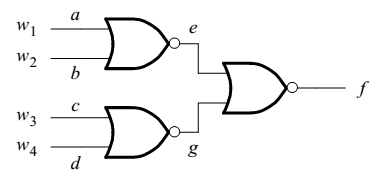
\includegraphics[scale=0.5]{Q1a.png}
	\end{center}
	
	Fault Test Table:
	\begin{center}
		\begin{adjustbox}{width=\columnwidth}
		\begin{tabular}{| c | c | c | c | c | c | c | c | c | c | c | c | c | c | c | c |}
			\hline
			Test & \multicolumn{14}{c |}{Faults that can be detected} \\
			\hline
			$w_1w_2w_3w_4$ & $a/0$ & $a/1$ & $b/0$ & $b/1$ & $c/0$ & $c/1$ & $d/0$ & $d/1$ & $e/0$ & $e/1$ & $g/0$ & $g/1$ & $f/0$ & $f/1$ \\
			\hline
			0000 & & & & & & & & & & & & & & \checkmark \\
			\hline
			0001 & & \checkmark & & \checkmark & & & & & \checkmark & & & & & \checkmark \\
			\hline
			0010 & & \checkmark & & \checkmark & & & & & \checkmark & & & & & \checkmark \\
			\hline
			0011 & & \checkmark & & \checkmark & & & & & \checkmark & & & & & \checkmark \\
			\hline
			0100 & & & & & & \checkmark & & \checkmark & & & \checkmark & & & \checkmark \\
			\hline
			0101 & & & \checkmark & & & & \checkmark & & & \checkmark & & \checkmark & \checkmark & \\
			\hline
			0110 & & & \checkmark & & \checkmark & & & & & \checkmark & & \checkmark & \checkmark & \\
			\hline
			0111 & & & \checkmark & & & & & & & \checkmark & & & \checkmark & \\
			\hline
			\hline
			1000 & & & & & & \checkmark & & \checkmark & & & \checkmark & & & \checkmark \\
			\hline
			1001 & \checkmark & & & & & & \checkmark & & & \checkmark & & \checkmark & \checkmark & \\
			\hline
			1010 & \checkmark & & & & & & & & & \checkmark & & \checkmark & \checkmark & \\
			\hline
			1011 & \checkmark & & & & & & & & & \checkmark & & & \checkmark & \\
			\hline
			1100 & & & & & & \checkmark & & \checkmark & & & \checkmark & & & \checkmark \\
			\hline
			1101 & & & & & & & \checkmark & & & & & \checkmark & \checkmark & \\
			\hline
			1110 & & & & & \checkmark & & & & & & & \checkmark & \checkmark & \\
			\hline
			1111 & & & & & & & & & & \checkmark & & \checkmark & \checkmark & \\
			\hline
		\end{tabular}
		\end{adjustbox}
	\end{center}
	
	Minimum Test Set: $\{0001, 0110, 1000, 1001\}$
	
	\subsection*{Part b}
	Label each wire as follows:
	
	\begin{center}
		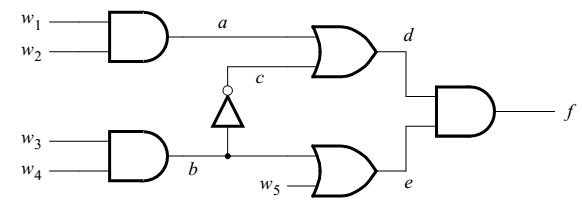
\includegraphics[scale=0.5]{Q1b.png}
	\end{center}
	
	There are seven paths:
	\begin{itemize}
		\item $w_1adf$, sensitized by $w_2w_3w_4w_5 = 111x$
		\item $w_2adf$, sensitized by $w_1w_3w_4w_5 = 111x$
		\item $w_3bcdf$, sensitized by $w_1w_2w_4w_5 = 0x11$
		\item $w_3bef$, sensitized by $w_1w_2w_4w_5 = 1110$
		\item $w_4bcdf$, sensitized by $w_1w_2w_3w_5 = 0x11$
		\item $w_4bef$, sensitized by $w_1w_2w_3w_5 = 1110$
		\item $w_5ef$, sensitized by $w_1w_2w_3w_4 = xx0x$
	\end{itemize}
	
	Minimum Test Set: $\{11110,01111,11100,11010,1011x,0x111,0x101\}$
	
	\section*{Question II}
	\subsection*{Part a}
	\begin{itemize}
		\item Input $0100$ detects $f/1$, $c/1$, $d/1$, $w_4/1$, $w_1/1$
		\item Input $0011$ detects $f/0$
		\item Input $0110$ detects $f/1$, $w_4/1$, $c/1$, $d/1$, $w_1/1$, $w_2/0$, $b/1$
		\item Input $1010$ detects $f/0$, $d/0$, $w_3/0$, $b/0$
		\item Input $1111$ detects $f/0$
	\end{itemize}
	
	We detected 11 faults of total 16 faults, so the percentage of simple fault are detected
	is:
	$$\frac{11}{16} \times 100\% = 68.75\%$$
	
	\subsection*{Part b}
	\begin{itemize}
		\item Input $1100$ detects $f/1$, $h/0$, $k/0$, $g/1$, $b/0$, $c/0$, $w_4/1$
		\item Input $0010$ detects $f/1$, $h/0$, $k/0$, $g/1$, $b/0$, $c/0$, $w_1/1$, $w_4/1$
		\item Input $0110$ detects $f/0$, $k/1$, $g/0$, $b/1$, $c/0$, $w_1/0$, $w_2/0$
	\end{itemize}
	
	\section*{Question III}
	Synchronous bus time consumption:
	\begin{enumerate}
		\item Send the address: 50 ns
		\item Read the memory: 200 ns
		\item Sending data to device: 50 ns
	\end{enumerate}
	Synchronous bus bandwidth:
	$$\frac{32\text{ bit}}{(50 + 200 + 50) \text{ ns}} = \frac{32 \times 10 ^ 9}{300 \times 2 ^ {20}}  \text{ Mbit/s} \approx 101.725 \text{ MBit/s}$$
	
	Asynchronous bus bandwidth:
	\begin{enumerate}
		\item ReadReq: 40 ns
		\item Read the memory: 200 ns
		\item Ack: $3 \times 40$ ns = 120 ns
	\end{enumerate}
	Asynchronous bus bandwidth:
	$$\frac{32\text{ bit}}{(40 + 200 + 120) \text{ ns}} = \frac{32 \times 10 ^ 9}{360 \times 2 ^ {20}}  \text{ Mbit/s} \approx 84.771 \text{ MBit/s}$$
\end{document}
